\documentclass{ctexart}
\usepackage{amsmath,amssymb,amsfonts}
\usepackage{authblk}
\renewcommand*{\Authsep}{, }
\renewcommand*{\Authand}{, }
\renewcommand*{\Authands}{, }
\usepackage{graphics}
\graphicspath{{figures/}}
\usepackage[url = false, doi = false, backend=biber,style=gb7714-2015,gbalign=gb7714-2015,gbpub=false,gbmedium=false]{biblatex}         
\usepackage{subfigure}
\usepackage{xcolor}
\usepackage{minted}
\colorlet{shadecolor}{gray!15}
\addbibresource{ref.bib}
\title{利用Qutip研究拉比振荡}
\author[1]{周子正}
\author[2]{朱哲昊}
\author[3]{孙蔚轩}
\affil[1]{物理科学学院, 南开大学}
\affil[2]{物理科学学院, 南开大学}
\affil[3]{金融学院, 南开大学}

\date{\today}

\begin{document}
\maketitle

\begin{abstract}
    拉比振荡广泛应用于量子计算、量子光学和凝聚态物理等领域。本文使用Qutip框架,对拉比振荡进行了数值计算,讨论了频率条件,RWA近似,衰减等影响,并利用数值方法拟合了振荡频率。
\end{abstract}

\textbf{关键词:} 拉比振荡\ 数值方法\ Qutip

\section{引言}
对于一个二能级系统,我们施加一个电磁波,在该电磁波频率恰当的场合,该系统中的原子会不断在$E_e$能级和$E_e$能级间跃迁,这种现象称之为拉比振荡\cite{zhu_vacuum_1990}。拉比振荡最早在核磁共振中发现,是核磁共振光谱法和核磁共振成像技术的基础,接受了大量实验的检验\cite{brune_quantum_1996}。广义地,它被定义为外场驱动下的一种周期性振荡现象,广泛应用于量子计算、量子光学和凝聚态物理等领域。考虑到拉比振荡中磁场或类磁场作用引起的时间反演对称破缺,手性应暗含在该动力学过程中。拉比振荡至今仍然有广泛的研究。
2020年,南开大学物理科学学院陈志刚教授、许京军教授领导的课题组理论研究发现,手性存在于拉比振荡的相位演化中\cite{zhang_unveiling_2020}。
\section{理论分析}
根据Jaynes - Fred Cummings 模型\cite{jaynes_comparison_1963}\cite{cummings_reminiscing_2013},在谐振器内的二能级原子体系的哈密顿量可以构造为:
\begin{equation}
    \hat{H}=\hbar \omega \hat{a}^{\dagger} \hat{a}+\hbar \omega_{0} \frac{\hat{\sigma}_{z}}{2}+\hbar g\left(\hat{a} +\hat{a}^{\dagger} \right)\left(\hat{\sigma}_{-}+\hat{\sigma}_{+}\right).
    \label{equ:H}
\end{equation}
其中,腔内光场的自作用项可以写成:
\begin{equation}
    \hat{H}_{photon}=\hbar \omega \hat{a}^{\dagger} \hat{a},
    \label{equ:photon}
\end{equation}
可以看成光子的量子模型,其中$\hat{a},\hat{a}^\dagger$是产生湮灭算符,$\hbar\omega$是能量最小单位。其表示与Quantum electrodynamics (QED)中的光子模型类似, 这个问题的模型被称为腔QED。对光子模型,其Fock空间下的表示为$\left|n\right>$。

类似的,可以证明,
\begin{equation}
    \hat{H}_{atom} = \hbar \omega_{0} \frac{\hat{\sigma}_{z}}{2},
\end{equation}
是原子的自作用哈密顿量,$\hbar\omega_0$是原子内部能级的能隙。其希尔伯特空间由$\left|e\right>,\left|g\right>$张成,与自旋$1/2$的费米子模型同构,其一组线性不相关完备算符族为$\hat{I},\hat{\sigma_z},\hat{\sigma_+},\hat{\sigma_-}$。用bra-ket表示为:
\begin{equation}
    \begin{aligned}
        \hat{I}        & = \left|g\right>\left<g\right|+\left|e\right>\left<e\right| \\
        \hat{\sigma_z} & = \left|g\right>\left<g\right|+\left|e\right>\left<e\right| \\
        \hat{\sigma_+} & = \left|g\right>\left<g\right|+\left|e\right>\left<e\right| \\
        \hat{\sigma_-} & = \left|g\right>\left<g\right|+\left|e\right>\left<e\right|
    \end{aligned}
    \label{equ:sigmas}
\end{equation}

二者的相互左用项由偶极子和外场的作用贡献
\begin{equation*}
    H_{int} = -\vec{d}\cdot\vec{E},
\end{equation*}
其算符表示相当于:
\begin{equation}
    \hat{H}_{int} = \hbar g\left(\hat{a} +\hat{a}^{\dagger} \right)\left(\hat{\sigma}_{-}+\hat{\sigma}_{+}\right)
\end{equation}
是相互作用项,$g$是耦合强度。当取$\delta  = \omega-\omega_0$趋于0时,体系的振动频率为$\Omega_r = 2g$,这就是拉比振荡的频率。体系的希尔伯特空间是光子和原子态空间的直积。

我们已经构造了完整的Hamiltonian,如Eq. \ref{equ:H}。类比费曼图,可以画出其中发生的四个过程:

\begin{figure}[htpb]
    \centering
    \subfigure[]{
        \centering
        \begin{minipage}[t]{0.45\linewidth}
            \centering
            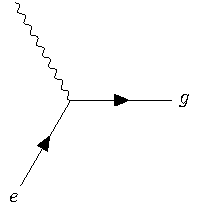
\includegraphics{fig1.pdf}
        \end{minipage}%
        \begin{minipage}[t]{0.45\linewidth}
            \centering
            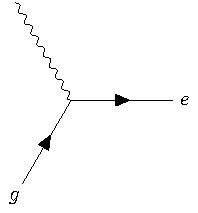
\includegraphics{fig2.pdf}
        \end{minipage}
    }\\
    \subfigure[]{
        \centering
        \begin{minipage}[t]{0.45\linewidth}
            \centering
            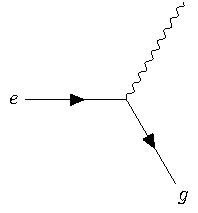
\includegraphics{fig3.pdf}
        \end{minipage}%
        \begin{minipage}[t]{0.45\linewidth}
            \centering
            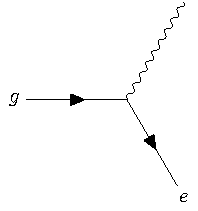
\includegraphics{fig4.pdf}
        \end{minipage}
    }%
    \caption{四种可能过程}
    \label{fig:4-process}
\end{figure}

图\ref{fig:4-process}中$\hat{a}^\dagger\sigma_+$和$\hat{a} \sigma_-$项的贡献在慢变场情况可以忽略,同时忽略双光子过程,可以将Eq. \ref{equ:H}约化为:
\begin{equation}
    \hat{H}_{RWA}=\hbar \omega \hat{a}^{\dagger} \hat{a}+\hbar \omega_{0} \frac{\hat{\sigma}_{z}}{2}+\hbar g\left(\hat{a}\hat{\sigma}_{+} +\hat{a}^{\dagger}\hat{\sigma}_{-} \right),
    \label{equ:H-RWA}
\end{equation}
这个结果和旋转波近似\cite{wu_strong-coupling_2007}相同。

\section{传统计算方法}
在研究具体系统与实验的对应时,传统的求解方法是要将初态$\left|\psi(0)\right> = C_g(0)\left|g\right> + C_e(0)\left|e\right>$将外场的形式带入薛定谔方程直接计算或者处理成微扰项进行近似计算。

在外场对时间只有平庸依赖$E = E_0 \exp(i\omega t)$的情况下可以写出其方程为:
\begin{equation}
    \begin{aligned}
        \frac{d}{d t} C_{e} & =-i \frac{\omega_{0}-\omega}{2} C_{e}-i \Omega_{r} C_{g} \\
        \frac{d}{d t} C_{g} & =+i \frac{\omega_{0}-\omega}{2} C_{g}-i \Omega_{r} C_{e}
    \end{aligned}
\end{equation}

若同时$\Omega_r$与时间无关时,此方程可以精确求解。其振动频率为$\Omega_r$。对于更加一般的问题,由于不能精确求解方程,处理方法是利用数值方法进行求解。

\section{Qutip计算方法}
\subsection{Qutip简介}
系统和外部世界之间总是存在着耦合,而且对系统进行的任何测量都必然涉及到与测量装置的耦合,因此会引入额外的外部影响。开发必要的理论和数值工具来解释系统与其环境之间的相互作用是理解实际量子系统动力学的重要步骤。
一般地,除了最基本的哈密顿量外,系统动力学的解析描述是不可能的,必须借助于运动方程的数值模拟。可以使用少量的effective oscillator和spin components来设计系统,其由有限数量的量子激发,可以在截断的希尔伯特空间中进行经典模拟。Python中的Quantum Toolbox(QuTiP)是一个用Python编程语言编写的开源框架\cite{johansson_qutip_2012}\cite{johansson_qutip_2013},旨在模拟上述系统的开放量子动力学。
QuTiP是一个开源软件,可以随意修改和使用。它基于Python脚本语言,易于阅读,可以快速生成代码,无需修改后再进行编译。QuTiP旨在提供各种用户友好的和高效的哈密顿量的数值模拟,包括具有任意时间依赖性的哈密顿量,还能使用优秀的Matplotlib包实现高质量绘图和动画的功能。

\subsection{利用Qutip构建系统的哈密顿量}
Qubit对无限维的光子场无法处理,在研究问题的背景下,其希尔伯特空间可以通过截断进行处理,此时可以定义出其哈密顿量为:

\begin{minted}[frame=lines,python3,mathescape,bgcolor=shadecolor]{python}
N = 50
#$\hat a$
a = tensor(destroy(N), qeye(2))
#$\hat \sigma$
sm = tensor(qeye(N), destroy(2))
#$\hat H$
isRWA = true #true or false
if isRWA:
    H = wc * a.dag() * a + wa * sm.dag() * sm \
    + 0.5 * wr * (a.dag() * sm + a * sm.dag())
else:
    H = wc * a.dag() * a + wa * sm.dag() * sm \
    + 0.5 * wr * (a.dag() + a) * (sm + sm.dag())
\end{minted}

初态定义为:

\begin{minted}[frame=lines,python3,mathescape,bgcolor=shadecolor]{python}
#$\left|\psi(0)\right>$
psi0 = tensor(basis(N, n), cg * basis(2, 0) \
    + ce * basis(2, 1))
\end{minted}

态随时间演化可以利用$mesolve$求出。特别的,实践中一般关注特定算符的期望值,算符的期望值随时间的演化可以直接求出。

mesolve的部分定义为:
\begin{minted}[frame=lines,python3,mathescape,bgcolor=shadecolor]{python}
def mesolve(H, initial_state, time_list, 
collapse_ops=None, expectation_ops=None)
\end{minted}

\subsection{拉比振荡的模拟}
首先对拉比振荡的条件进行检验,当失谐$\delta = \omega_0 - \omega$不趋近于0时,拉比振荡不会发生,此情况可以模拟为:

\begin{minted}[frame=lines,python3,mathescape,bgcolor=shadecolor]{python}
wc = 1.0 * 2 * np.pi
wa = 1.5 * 2 * np.pi
wr = 0.07 * 2 * np.pi
H = Get_H_operator(wc, wa, wr, True)
psi0 = Get_initial_state(0, 1, 0)
tlist = np.linspace(0, 25, 100)
c_op_list = Get_c_ops(0, 0, 0)
output = mesolve(H, psi0, tlist, c_op_list,\
 [a.dag() * a, sm.dag() * sm])
\end{minted}

结果为图。
\begin{figure}[htbp]
    \begin{minipage}[t]{0.5\linewidth}
        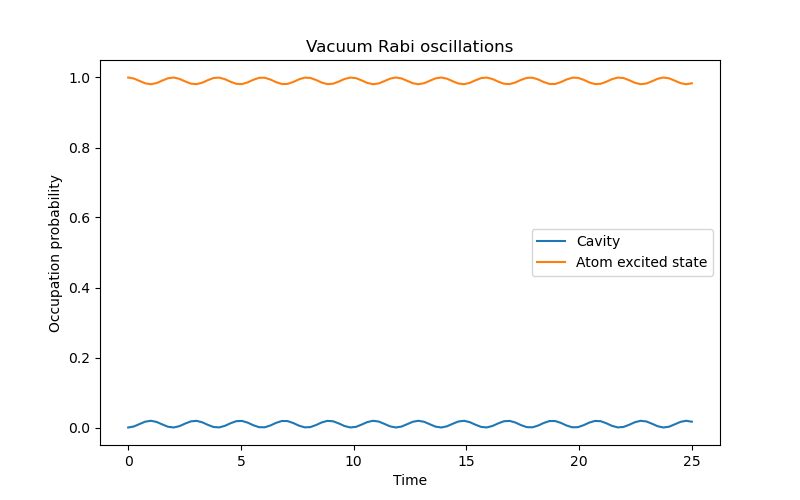
\includegraphics[width=0.7\linewidth]{1.png}
        \caption{振荡频率条件破坏}
        \label{fig:1}
    \end{minipage}%
    \begin{minipage}[t]{0.5\linewidth}
        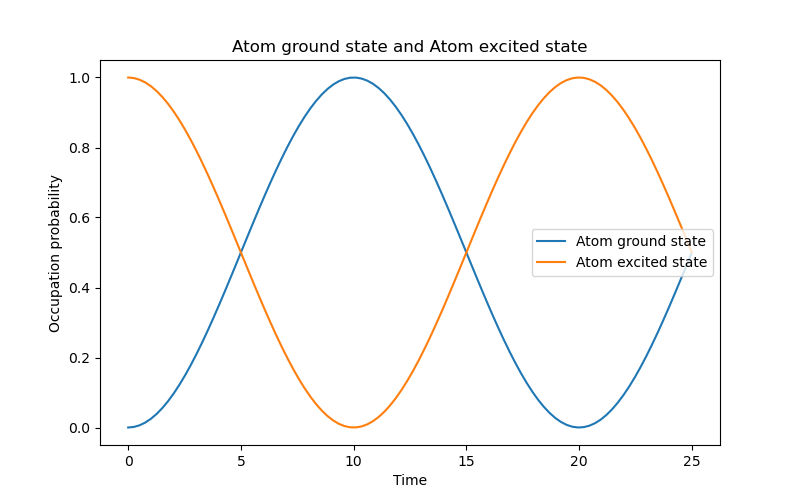
\includegraphics[width=0.7\linewidth]{2.png}
        \caption{基态和激发态之间的能量传递}
        \label{fig:2}
    \end{minipage}
\end{figure}


可以看出,此时拉比振荡没有发生。

当失谐取0时,可以对拉比振荡进行求解,作为一个示例,取初态原子全部处于激发态,光场不携带能量。

从图可以看到,能量在两个激发态和基态之间跃迁,同时在光场和原子之间交换。

振荡的形式类似于三角函数,通过拟合可以求出其振荡频率。

拟合出的振荡频率为,与参数相符,证明模拟是正确的。

旋转波近似实际上只适用于低频情况,通过图 可以看到,在高频条件下旋转波近似结果与实际结果偏离很大。
\subsection{耗散效应}
实际实验中包含了各种情况的耗散,耗散也可以利用Qutip框架进行计算。耗散过程的算符可以定义为:

带有耗散的计算给出的结果如图所示

可以看到,耗散导致总能量衰减,振幅减弱。
\section{结论}
拉比振荡的传统计算方法是采用数值法求解微分方程。本文使用python语言,利用Qutip框架,根据Jaynes - Fred Cummings 模型计算出拉比振荡随时间的演化。
我们验证了拉比振荡的频率条件,RWA近似的使用范围,对拉比振荡进行了模拟与可视化,通过数据分析方法验证了拉比振荡的频率结果。
\section{参考文献}
\printbibliography[heading=none]
\end{document}